\section{Results}\label{sec:results}
\IfFileExists{tables/tab_main.tex}{\begin{table*}[t]
\centering
\caption{Main results over \val{NseedsRun} paired seeds (\%). Net ASR $=$ ASR $-$ ASR of the paraphrase placebo, with 95\% bootstrap CIs. \emph{Adaptive}: MisGen's feedback loop runs against the defended agent. \emph{Frozen}: the attack recorded against the undefended agent is replayed verbatim. Clean return is the paired clean agent's cumulative return over the 60-day window; drawdown is the attacked agent's maximum drawdown.}
\label{tab:main}
\small
\setlength{\tabcolsep}{4.5pt}
\begin{tabular}{@{}lrrrrrrr@{}}
\toprule
Defence & MER & ASR & Placebo ASR & Net ASR (adaptive) & Net ASR (frozen) & Clean return & Drawdown \\
\midrule
No defence & 62.1 & 39.3 & 20.9 & 18.4 [16.6, 20.1] & 18.4 [16.6, 20.1] & +6.6 & $-$4.8 \\
Grounding & 59.5 & 21.6 & 14.2 & 7.4 [6.2, 8.6] & 8.4 [7.1, 9.7] & +2.9 & $-$5.9 \\
Grounding + risk & 59.5 & 26.8 & 17.5 & 9.3 [7.8, 10.9] & 9.0 [7.6, 10.4] & +2.2 & $-$5.6 \\
\bottomrule
\end{tabular}
\end{table*}
}{}

\subsection{Effect of the defense layer}\label{sec:results-effect}
Against the undefended agent the adaptive attack reaches an MER of \val{MInjectedNoneMER}\% and a naive ASR of \val{MInjectedNoneASR}\% (Table~\ref{tab:main}); after subtracting the placebo, its misinformation-driven (net) ASR is \val{CmpNetNone}\% \ci{CmpNetNone}. Temporal grounding lowers net ASR by \cmp{CmpGainAdaptiveGroundedNet} against the adaptive attacker (\pholm{CmpGainAdaptiveGroundedNet}) and by \cmp{CmpGainFrozenGroundedNet} against the frozen one (\pholm{CmpGainFrozenGroundedNet}), so the benefit does not depend on the attacker adapting. It also cuts placebo-corrected active flips, the trades the attacker changed, by \cmp{CmpGainAdaptiveGroundedActnet} (\pholm{CmpGainAdaptiveGroundedActnet}). Because each arm is corrected with its own placebo, this gain is not an artifact of grounding making the agent less sensitive to \emph{any} change in its news pool, although it does that too. The full layer, grounding plus risk layer, lowers net ASR by \cmp{CmpGainAdaptiveGroundedRiskNet} (adaptive) and \cmp{CmpGainFrozenGroundedRiskNet} (frozen): still a large gain, but smaller than grounding alone (Sec.~\ref{sec:results-components}).

\begin{figure}[t]
\centering
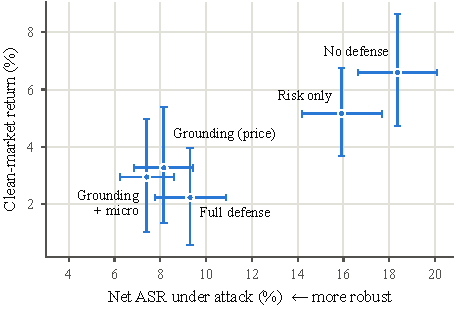
\includegraphics[width=\columnwidth]{figures/fig_frontier.pdf}
\caption{Robustness--return frontier: net ASR under the adaptive attack against the clean-market return of the same defense (mean and 95\% CIs over \val{NseedsRun} seeds). Grounding moves the agent left at a cost in return; microstructure proxies and the risk layer do not move it further.}
\label{fig:frontier}
\end{figure}

The defense does not neutralize the attack: the grounded agent's net ASR is still \val{CmpNetGrounded}\% \ci{CmpNetGrounded}. Its price is \cmp{CmpCostGrounded} of clean-market return, and \cmp{CmpCostGroundedRisk} for the full layer (Fig.~\ref{fig:frontier}). The synthetic news is genuinely informative, and grounding discounts true stories that the lagging market evidence does not yet support. Under one identical recorded attack (Appendix~\ref{app:example}), the undefended agent and its twin disagree on \val{ReplayFlipsNone} of \val{ReplayDays} days, and the grounded agent and its twin on \val{ReplayFlipsGrounded}.

\textbf{How much of the attack is misinformation?} The placebo alone, paraphrases that change no fact, flips \val{MPlaceboNoneASR}\% of the undefended agent's decisions. The matched controls attribute the rest (Appendix~\ref{app:ladder}): the attacker's bias prompts add \cmp{CmpDecBiasNone}, and the content of the misinformation adds \cmp{CmpDecMeaningNone}, about \val{ShareMeaningOfNaive}\% of the naive ASR. Grounding lowers both the noise floor, cutting placebo ASR by \cmp{CmpPlaceboGrounded}, and the content effect, to \cmp{CmpDecMeaningGrounded}.

\subsection{Comparison with standard defenses}\label{sec:results-baselines}
\IfFileExists{tables/tab_baselines.tex}{\begin{table}[t]
\centering
\caption{Grounding and standard defenses (mean over 100 seeds, \%): ASR and net ASR under the adaptive attack, net ASR under its frozen replay, clean-market return (CR) over the evaluation window, and the shares of injected and of clean retrieved documents that the detection filter drops. The attacker screens its candidates with the same detector at a 10\% false-positive rate.}
\label{tab:baselines}
\footnotesize
\begin{adjustbox}{max width=\linewidth}
\begin{tabular}{lrrrrrr}
\toprule
 & & \multicolumn{2}{c}{Net ASR} & & \multicolumn{2}{c}{Dropped} \\
\cmidrule(lr){3-4}\cmidrule(lr){6-7}
Defense & ASR & Adapt. & Frozen & CR & Inj. & Clean \\
\midrule
No defense & 39.3 & 18.4 & 18.4 & 6.6 & -- & -- \\
Ignore the news & 0.0 & 0.0 & 0.0 & $-$0.3 & -- & -- \\
Detection filter, 10\% FPR & 38.9 & 16.5 & 17.0 & 6.0 & 0.0 & 10.2 \\
Detection filter, 25\% FPR & 40.6 & 15.5 & 15.7 & 5.9 & 13.3 & 25.1 \\
Weighted median & 35.5 & 12.4 & 12.9 & 6.7 & -- & -- \\
Trimmed mean & 35.1 & 15.1 & 15.8 & 7.1 & -- & -- \\
Temporal grounding & 21.6 & 7.4 & 8.3 & 2.9 & -- & -- \\
\bottomrule
\end{tabular}
\end{adjustbox}
\end{table}}{}
Of all defenses that still read the news, grounding leaves the lowest net ASR (Table~\ref{tab:baselines}). Ignoring the news removes the attack surface but also the information in the news. It costs \cmp{CmpBaseCostTextFree} of clean return, against \cmp{CmpBaseCostGrounding} for grounding.

\textbf{Detection filtering fails against a screening attacker.} At a 10\% flag rate the filter drops \val{AblBaselinesInjectedDetectOneZeroFilterRecall}\% of the injected documents, because MisGen already discards every candidate that the detector flags at this rate, but it drops \val{AblBaselinesCleanDetectOneZeroFilterCleanDrop}\% of genuine news. At 25\% it drops \val{AblBaselinesInjectedDetectTwoFiveFilterRecall}\% of injected and \val{AblBaselinesCleanDetectTwoFiveFilterCleanDrop}\% of genuine documents. The agent then reads more misinformation (MER \val{AblBaselinesInjectedNoneMER}\% $\to$ \val{AblBaselinesInjectedDetectTwoFiveMER}\%), and its ASR does not fall. Its net ASR still falls, by \cmp{CmpBaseAdaptiveDetectTwoFive}, but only because the filter's own drops make the twins disagree more even when the injected documents are harmless paraphrases: placebo ASR rises from \val{AblBaselinesPlaceboNoneASR}\% to \val{AblBaselinesPlaceboDetectTwoFiveASR}\%. Net ASR thus flatters a defense that makes the agent noisier. Grounding does the opposite: it lowers placebo ASR, so its raw gain (\cmp{CmpGainAdaptiveGroundedAsr}) exceeds its net gain. If the attacker does not screen its candidates, the 25\% filter drops \val{AblBaselinesInjectedDetectTwoFiveNofilterFilterRecall}\% of injected documents. It then lowers net ASR by \cmp{CmpBaseFrozenDetectNofilter} on the replayed attack, but not detectably once the attacker adapts (\cmp{CmpBaseAdaptiveDetectNofilter}).

\textbf{Robust aggregation helps less than grounding.} The weighted median lowers net ASR by \cmp{CmpBaseAdaptiveMedian} at no detectable cost (\cmp{CmpBaseCostMedian}), and the trimmed mean by \cmp{CmpBaseAdaptiveTrimmed}. Grounding lowers it by a further \cmp{CmpBaseAdaptiveMedianVsGrounding} beyond the median (\pholm{CmpBaseAdaptiveMedianVsGrounding}). With an MER of \val{AblBaselinesInjectedNoneMER}\%, injected documents are most of what the agent reads, beyond the 50\% breakdown point of the median. Grounding needs no clean majority, because its reference is the market.

\subsection{Does grounding generalize?}\label{sec:results-general}
\begin{figure}[t]
\centering
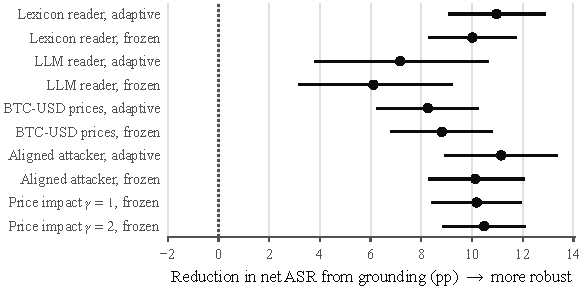
\includegraphics[width=\columnwidth]{figures/fig_generalization.pdf}
\caption{Grounding's reduction in net ASR in every setting we test (points: mean per-seed reduction; bars: 95\% bootstrap CIs; filled: detectable after Holm correction). Seeds: \val{NseedsLlmr} for the LLM reader, \val{NseedsReal} for BTC-USD, and \val{NseedsRun} otherwise.}
\label{fig:generalization}
\end{figure}
Grounding's gain is detectable in every setting we test (Fig.~\ref{fig:generalization}).

\textbf{A local LLM reader.} With \texttt{\val{LlmrModel}} scoring the news, the undefended agent's net ASR is \val{CmpLlmrNetNone}\% \ci{CmpLlmrNetNone}. Grounding lowers it to \val{CmpLlmrNetGrounded}\%, a gain of \cmp{CmpLlmrGainAdaptiveGroundedNet}, for \cmp{CmpLlmrCostGrounded} of clean return; against the replay the gain is \cmp{CmpLlmrGainFrozenGroundedNet}. The decomposition carries over. The misinformation's content adds \cmp{CmpLlmrDecMeaningNone} to the undefended agent's ASR and \cmp{CmpLlmrDecMeaningGrounded} to the grounded agent's. As with the lexicon, adding the risk layer does not lower net ASR further (\cmp{CmpLlmrGainAdaptiveRiskNet}).

\textbf{Real prices.} On \val{NseedsReal} BTC-USD windows, grounding lowers net ASR from \val{CmpRealNetNone}\% to \val{CmpRealNetGrounded}\% (\cmp{CmpRealGainAdaptiveGroundedNet}; frozen: \cmp{CmpRealGainFrozenGroundedNet}). It costs \cmp{CmpRealCostGrounded} of the \val{RealCleanNoneCR}\% that the undefended agent earns per window in a clean market.

\textbf{Attackers that know the defense.} The evidence-aligned attacker gains nothing. Its net ASR differs from the standard attacker's by \cmp{CmpAwareAdaptiveAlignedVsStdNone} without a defense and by \cmp{CmpAwareAdaptiveAlignedVsStdGrounding} with grounding, and grounding's gain does not shrink (\cmp{CmpAwareAdaptiveGainDropAligned}). Presumably, edits that agree with the market push the agent where the evidence already points, so they rarely change a decision. The conflict-seeking attacker is stronger: against the full layer it raises net ASR by \cmp{CmpAwareAdaptiveConflictVsStdFull} (\pholm{CmpAwareAdaptiveConflictVsStdFull}).

\textbf{Misinformation that moves prices.} When the replayed attack also moves prices, grounding's gain is \cmp{CmpImpGainGroundedOnepZero} at $\gamma=1$ and \cmp{CmpImpGainGroundedTwopZero} at $\gamma=2$. Neither differs detectably from $\gamma=0$ (\cmp{CmpImpGainDropTwopZero} at $\gamma=2$). Both twins trade the moved prices, so ASR here measures what reading the fake text adds to its price effect. A defense grounded in prices cannot undo a real price move; it can only stop the agent from acting on the text alone.

\begin{figure}[t]
\centering
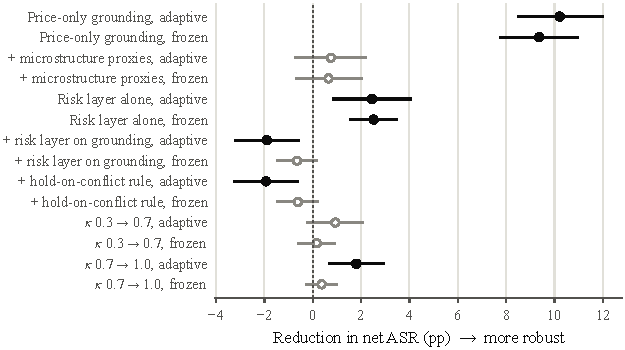
\includegraphics[width=\columnwidth]{figures/fig_forest.pdf}
\caption{Effect of each defense component on net ASR over \val{NseedsRun} seeds (points: mean per-seed reduction; bars: 95\% bootstrap CIs; filled: detectable after Holm correction). Positive is more robust. Rows starting with ``+'' add one component: the proxies to price-only grounding, the risk layer to grounding, and the hold-on-conflict rule to the rest of the risk layer.}
\label{fig:forest}
\end{figure}

\subsection{Which components matter}\label{sec:results-components}
\textbf{Price-based grounding does the work.} Price-only grounding alone lowers net ASR by \cmp{CmpAblDefAdaptiveGrounding} (Fig.~\ref{fig:forest}). Adding the microstructure proxies changes it by \cmp{CmpAblDefAdaptiveMicro} (adaptive) and \cmp{CmpAblDefFrozenMicro} (frozen), neither detectable. In our generator, high, low and volume are functions of the simulated return and volatility plus independent noise, so the proxies carry no directional information beyond the price path. Grounding strength matters little: only the step from $\kappa=0.7$ to $1.0$ against the adaptive attacker lowers net ASR detectably (\cmp{CmpAblKappaAdaptiveZeropSevenOnepZero}, \pholm{CmpAblKappaAdaptiveZeropSevenOnepZero}), and each step costs about \val{CmpAblKappaCostZeropSevenOnepZero}\pp{} of clean return.

\textbf{The risk layer can backfire.} On its own the risk layer lowers net ASR by \cmp{CmpAblDefAdaptiveRiskAlone} (\pholm{CmpAblDefAdaptiveRiskAlone}). On top of grounding, however, it \emph{raises} net ASR against the adaptive attacker by \cmpneg{CmpGainAdaptiveRiskNet} (\pholm{CmpGainAdaptiveRiskNet}) and placebo-corrected active flips by \cmpneg{CmpGainAdaptiveRiskActnet}, with no detectable drawdown benefit (\cmp{CmpDdRisk}, \pholm{CmpDdRisk}). The hold-on-conflict rule accounts for the increase: removing it lowers net ASR by \cmpneg{CmpAblDefAdaptiveHold} (\pholm{CmpAblDefAdaptiveHold}). Injected text creates a text--market conflict on exactly the days it is injected, so holding on conflict changes the attacked agent's decision on those days, while its clean twin, reading genuine news, trades as usual. The attacker thereby decides when the rule fires. Against the frozen attack the change in net ASR from adding the risk layer is not detectable (\cmp{CmpGainFrozenRiskNet}).

\textbf{Shrink instead of hold.} A conflict should change the size of a trade, not its direction. Replacing hold-on-conflict with shrink-on-conflict lowers the full layer's net ASR from \val{AblConflictHandlingInjectedHoldASRNet}\% to \val{AblConflictHandlingInjectedShrinkASRNet}\% (\cmp{CmpConfAdaptiveShrinkAsrNet}, \pholm{CmpConfAdaptiveShrinkAsrNet}), the level of grounding alone (\val{AblDefenseInjectedGroundingMicroASRNet}\%), and as much as dropping the rule (\cmp{CmpConfAdaptiveNoholdAsrNet}). It also narrows the mean gap between the twins' positions by \cmp{CmpConfAdaptiveShrinkPositionGap}. Against the conflict-seeking attacker, shrinking helps by \cmp{CmpConfAdaptiveConflictShrinkAsrNet}. That attacker's advantage does not come from the conflict rule, however: it gains \cmp{CmpConfAdaptiveAttackerShrink} under shrinking and \cmp{CmpConfAdaptiveAttackerNohold} with no conflict rule at all.
